\documentclass[11pt]{beamer}
\usetheme{Warsaw}
\usepackage[utf8]{inputenc}
\usepackage[brazil]{babel}  % idioma
\usepackage{amsmath,amsfonts,amssymb,textcomp}
\usepackage{graphicx}
\usepackage{subfigure}

\author{Othon Oliveira}
\title{Sistemas Operacionais}
%\setbeamercovered{transparent} 
%\setbeamertemplate{navigation symbols}{} 
%\logo{} 
\institute{Fatec -- Faculdade de Informática --- PE} 
%\date{} 
%\subject{} 
\begin{document}


% Capa - requer o TikZ
\newcommand{\capa}{
    \begin{tikzpicture}[remember picture,overlay]
        \node at (current page.south west)
            {\begin{tikzpicture}[remember picture, overlay]
                \fill[shading=radial,top color=orange,bottom color=orange,middle color=yellow] (0,0) rectangle (\paperwidth,\paperheight);
            \end{tikzpicture}
          };
    \end{tikzpicture}
}


\begin{frame}
\titlepage
\end{frame}

%\begin{frame}
%\tableofcontents
%\end{frame}



%+++++++++++++++++++++++++++++++++++++++++++++++
\begin{frame}{Threads -- Conceito}
\begin{figure}[h]
%\left

\includegraphics[width=18mm, height=15mm]{Figuras/appleOficial.jpg}
\qquad \quad \quad \quad \quad

\includegraphics[width=19mm, height=17mm]{Figuras/windows.png}
\qquad \quad \quad \quad \quad \quad \quad 	\vspace{1.0in}

\includegraphics[width=15mm, height=15mm]{Figuras/android.jpg}
\qquad \quad \quad \quad \quad \quad \quad \quad 

\includegraphics[width=25mm, height=15mm]{Figuras/ubuntu_904.jpg}

\end{figure}
\end{frame}

%+++++++++++++++++++++++++++++++++++++++++++++++
\section{Threads}
\subsection*{Conceito}

\begin{frame}{Espaço de endereçamento}
 Em sistemas tradicionais, cada processo tem um espaço de endereçamento e um único Thread (fluxo) de controle.
 \begin{block}{Definição}
 	Isso é quase uma definição de processo, exceto pelo espaço de endereçamento
 \end{block}
 Contudo é frequente querer ter múltiplos threads em um único espaço de endereçamento executando em quase-paralelamente, como se fossem processos separados.
\end{frame}


\begin{frame}\frametitle{ Múltiplos processos com múltiplas threads}

\begin{columns}

\begin{column}{0.01cm}
\begin{figure}[ht]
\begin{center}
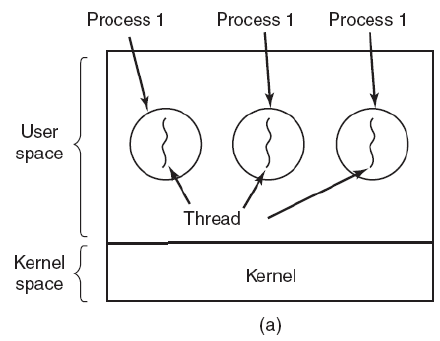
\includegraphics[height=3.3cm]{Figuras/process-thread1.png}
%\caption{Estados -- simplificado}
\end{center}

\end{figure}
\end{column}

\pause

\begin{column}{0.01cm}
\begin{figure}[ht]
\begin{center}
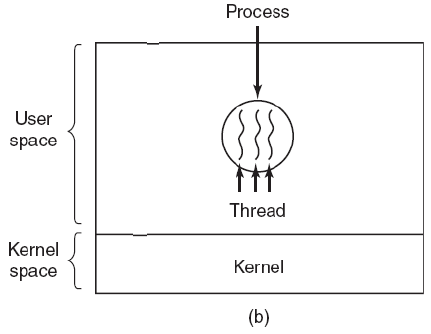
\includegraphics[height=3.5cm]{Figuras/process-thread3.png}
%\caption{Máquina de estados finitos -- completo}
\end{center}
\end{figure}
\end{column}

\end{columns}
Em qual das figuras há multithread ?

\pause

\begin{block}{Multithread}
 Multithread também é usado para descrever múltiplos threads em um único processo
\end{block}

\end{frame}


%\subsection*{Trabalho de Pesquisa}

\begin{frame}\frametitle{ Threads de ambiente}


\begin{block}{ Independência entre Threads}
O que as Threads acrescentam ao modelo de processo é permitir que múltiplas execuções ocorram no mesmo ambiente do processo, com um grande grau de independência.
\end{block}
Na figura (a) vemos três processos tradicionais. Cada um possui seu próprio espaço de endereçamento e um único thread e controle.

Na figura (b) vemos um único processo com três threads de controle.

Quantos threads há nos dois casos ??

\end{frame}

%+++++++++++++++++++++++++++++++++++++++++++++++
\begin{frame}\frametitle{ Threads de ambiente}

\begin{block}{ Espaço de endereçamento}

Na figura (a) cada processo tem seu próprio seu espaço de endereçamento diferente.
Já na figura (b) todos os três threads compartilham o mesmo endereçamento.

%voltar para ver a figura novamente
\end{block}

Quando um processo com múltiplas threads é executado, em um sistema com uma única CPU, os threads esperam a vez de executar.

\end{frame}


%+++++++++++++++++++++++++++++++++++++++++++++++
\begin{frame}\frametitle{ A pilha de Threads}

\begin{block}{ A pilha de Threads}
\begin{table}[htbp]
 \scriptsize
%      \centering  \caption{Cronograma -- 12 meses}
	\begin{tabular}{|l|c|c}
	\hline
	\textbf{Itens por processo} & \textbf{Itens por threads}  \\
	  \hline
	  Espaço de endereçamento & Contador de programas \\ \hline
	  Variáveis globais & Registradores \\ \hline
	  Arquivos abertos & Pilha \\ \hline
	  Processos filhos & Estado \\ \hline
	  Alarmes pendentes & ---  \\ \hline
	  Sinais e tratadores de sinais & --- \\ \hline
	  Informações de contabilidade & --- \\ \hline
	\end{tabular}
\end{table}
\end{block}

\pause
A primeira coluna relaciona alguns itens compartilhados por todos os threads em um processo.
A segunda mostra alguns itens privativos de cada thread.

\end{frame}
%+++++++++++++++++++++++++++++++++++++++++++++++
\section{Uso de threads}
\subsection{Por quê usar threads}

\begin{frame}\frametitle{ Por quê usar threads?}

\begin{block}{ 1º uso de Threads}
O modelo de programação se torna mais simples se decompormos uma aplicação em múltiplos threads sequencias que executam quase-paralelo.
\end{block}

\pause

\begin{block}{2º uso de Threads}
 Threads são mais fáceis de criar e destruir que os processos, por quê?
 \pause
 Não têm qualquer recurso associado a eles.
\end{block}

\pause

\begin{block}{3º uso de Threads}
 Threads são úteis em sistemas com múltiplas CPUs, para os quais o paralelismo é possível.
\end{block}

\end{frame}

%+++++++++++++++++++++++++++++++++++++++++++++++
\begin{frame}\frametitle{ Exemplo}
\begin{block}{Um processador de textos}
 Um processador de textos que salva automaticamente o arquivo a medida que o usuário vai digitando tem, no mínimo quantas threads?
\end{block}

\end{frame}

%+++++++++++++++++++++++++++++++++++++++++++++++
\begin{frame}{Um processador de textos com múltiplas threads}
\begin{figure}[h]

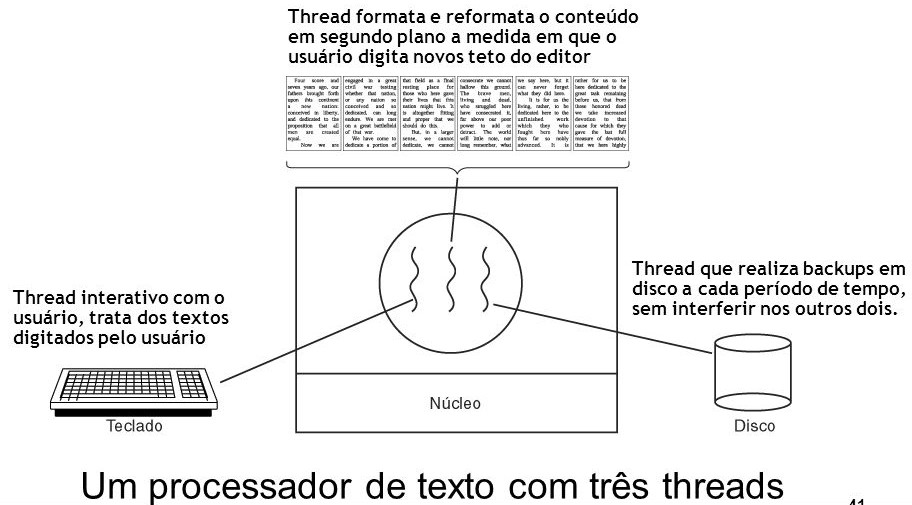
\includegraphics[width=100mm, height=60mm]{Figuras/threadsTexto.jpg}

\end{figure}
\end{frame}


%+++++++++++++++++++++++++++++++++++++++++++++++

\begin{frame}{ Um servidor Web multithreads}
\begin{figure}[h]

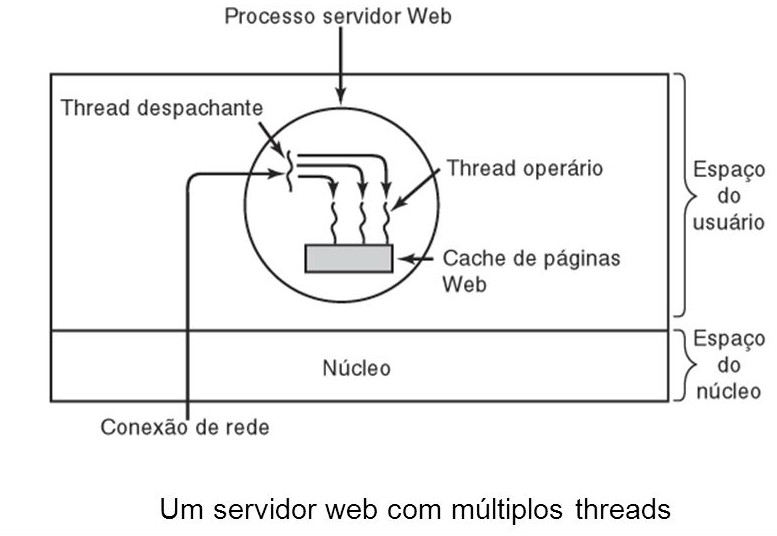
\includegraphics[width=100mm, height=60mm]{Figuras/threadsServidor.jpg}
\end{figure}

\end{frame}


%+++++++++++++++++++++++++++++++++++++++++++++++
\begin{frame}\frametitle{ Exemplo}

\begin{block}{ Um servidor Web multithreads}
Um modo de organizar o servidor Web é mostrado na figura acima.
Na figura, um thread, o \textbf{despachante}, lê as requisições que chegam à rede. Depois de examinar a requisição, ele escolhe um thread \textbf{operário} ocioso (isto é bloqueado) e entrega-lhe a requisição, possivelmente com um ponteiro associado a mensagem e uma palavra especial para cada thread. Na prática o despachante ``acorda'' o operário que está descansando, tirando-o do estado bloqueado e colocando-o no estado pronto.
\end{block}

\end{frame}

%+++++++++++++++++++++++++++++++++++++++++++++++
%\begin{frame}\frametitle{ Exemplo}

%\begin{block}{ Um servidor Web monothread}
%\begin{tabular}{Thread despachante}
%	while(true)\{\\
%		get_next_request(&buf);\\
%		handoff_work(&buf);\\
%	\}
%\end{tabular}
%\end{block}

%\pause

%\begin{block}{ Um servidor Web monothread}
%$while(true){
%	wait_for_work(&buf);
%	look_for_page_in_cache(&buf, &page);
%	if(page_not_in_cache(&page)) read_page_from_disk(&buf, &page);
%	return_page(&page);
%}
%Thread operário
%\end{block}

%\end{frame}

%+++++++++++++++++++++++++++++++++++++++++++++++

%+++++++++++++++++++++++++++++++++++++++++++++++

%+++++++++++++++++++++++++++++++++++++++++++++++

%+++++++++++++++++++++++++++++++++++++++++++++++


%+++++++++++++++++++++++++++++++++++++++++++++++

%+++++++++++++++++++++++++++++++++++++++++++++++



\end{document}